\documentclass[fleqn, a4paper, 11pt, oneside]{amsart}
%\usepackage[top = 2cm, bottom = 1cm, left = 1cm, right = 1cm]{geometry}
\usepackage{exsheets, tasks}
\usepackage{amsmath, amssymb, amsthm} %standard AMS packages
\usepackage{marginnote} %marginnotes
\usepackage{gensymb} %miscellaneous symbols
\usepackage{commath} %differential symbols
\usepackage{xcolor} %colours
\usepackage{cancel} %cancelling terms
\usepackage[free-standing-units, space-before-unit]{siunitx} %formatting units
	\sisetup
	{
		per-mode=fraction,
		fraction-function=\frac
	}
\usepackage{tikz, pgfplots} %diagrams
\usetikzlibrary{calc, hobby, patterns, intersections, decorations.markings}
\usepackage{graphicx} %inserting graphics
\usepackage{hyperref} %hyperlinks
\usepackage{datetime} %date and time
\usepackage{ulem} %underline for \emph{}
\usepackage{xfrac} %inline fractions
\usepackage{enumerate,enumitem} %numbered lists
\usepackage{float} %inserting floats
\usepackage{circuitikz}[american voltages, american currents] %circuit diagrams
\usepackage[utf8]{inputenc}
\usepackage{booktabs}
\usepackage{todonotes}

\newcommand\numberthis{\addtocounter{equation}{1}\tag{\theequation}} %adds numbers to specific equations in non-numbered list of equations

\newcommand{\AxisRotator}[1][rotate=0]{
	\tikz [x=0.25cm,y=0.60cm,line width=.2ex,-stealth,#1] \draw (0,0) arc (-150:150:1 and 1);%
} %rotation symbols on axes

\theoremstyle{definition}
\newtheorem{example}{Example}
\newtheorem{definition}{Definition}

\theoremstyle{theorem}
\newtheorem{theorem}{Theorem}

\newcommand{\curl}{\mathrm{curl\,}}

\makeatletter
\@addtoreset{section}{part} %resets section numbers in new part
\makeatother

\renewcommand{\thesubsection}{(\arabic{subsection})}
\renewcommand{\thesection}{(\arabic{section})}

\renewcommand{\emph}{\uline}

\renewcommand{\tilde}{\widetilde}

%section headings on left
\makeatletter
\def\specialsection{\@startsection{section}{1}%
	\z@{\linespacing\@plus\linespacing}{.5\linespacing}%
	%  {\normalfont\centering}}% DELETED
	{\normalfont}}% NEW
\def\section{\@startsection{section}{1}%
	\z@{.7\linespacing\@plus\linespacing}{.5\linespacing}%
	%  {\normalfont\scshape\centering}}% DELETED
	{\normalfont\scshape}}% NEW
\makeatother

%forces newline after subsection
\makeatletter
\def\subsection{\@startsection{subsection}{3}%
	\z@{.5\linespacing\@plus.7\linespacing}{.1\linespacing}%
	{\normalfont\itshape}}
\makeatother

\settasks{counter-format = tsk[1].}

\SetupExSheets{solution/print = true}

%opening
\title{Quantum and Solid State Physics : Assignment 8}
\author
{
	Aakash Jog\\
	ID : 989323563
}
\date{\formatdate{17}{12}{2015}}

\begin{document}

\tikzset{->-/.style={decoration={
  markings,
  mark=at position #1 with {\arrow{>}}},postaction={decorate}}}

\maketitle
%\setlength{\mathindent}{0pt}

\begin{question}
	\begin{enumerate}
		\item
			The hole concentration of Si at $T = 300 \kelvin$ increases linearly from $x = 0 \si{\centi\metre}$ to $x = 0.01 \si{\centi\metre}$.
			At $x = 0 \si{\centi\metre}$, the hole concentration is $p = 4 \times 10^{17} \si{\per\centi\metre\cubed}$.
			The hole diffusion coefficient is $D_p = 10 \si{\centi\metre\squared\per\second}$.
			The magnitude of hole diffusion current density is $J_{\text{diffusion}_p} = 20 \si{\ampere\per\centi\metre\squared}$.
			Determine the hole concentration at $x = 0.01 \si{\centi\metre}$.
		\item
			The electron concentration in a sample of silicon is given by
			\begin{align*}
				n(x) &= 10^{15} e^{-\frac{x}{L_n}} \si{\per\centi\metre\cubed}
			\end{align*}
			where $L_n = 10^{-4} \si{\centi\metre}$, and $0 \le x < \infty$.
			The electron diffusion coefficient is $D_n = 25 \si{\centi\metre\squared\per\second}$.
			Draw the electron concentration profile as a function of distance, and indicate the direction of electron flow, and of electron current density $J_{\text{diffusion}_n}$ on the figure.
			Determine the electron diffusion current density $J_{\text{diffusion}_n}$ at $x = 0$, $x = L_n$, and as $x \to \infty$.
			Mathematically, what is the significance of $L_n$?
			Answer this by comparing electron concentration at $x = L_n$ to its initial value at $x = 0$.
			At $x = L_n$, $n(x)$ has decayed to what fraction of its initial value?
	\end{enumerate}
\end{question}

\begin{solution}
	\begin{enumerate}[leftmargin=*]
		\item
			\begin{align*}
				J_{\text{diffusion}_p} &= q D_p \dod{p}{x}\\
				\therefore 20 \si{\ampere\per\centi\metre\squared} &= (q) \left( 10 \si{\centi\metre\squared\per\second} \right) \dod{p}{x}\\
				\therefore \frac{2}{q} \si{\ampere\second} &= \dod{p}{x}
			\end{align*}
			Therefore,
			\begin{align*}
				\frac{p_0 - p_{0.01}}{0 - 0.01} &= \frac{2}{q}\\
				\therefore \frac{p_0 - p_{0.01}}{0.01} &= -\frac{2}{1.6} \times 10^{19}\\
				\therefore p_0 - p_{0.01} &= -1.25 \times 10^{17}\\
				\therefore p_{0.01} &= 4 \times 10^{17} + 1.25 \times 10^{17}\\
				&= 5.25 \times 10^{17}
			\end{align*}
		\item
			\begin{align*}
				n(x) &= 10^{15} e^{-\frac{x}{L_n}}
			\end{align*}
			Therefore,
			\begin{align*}
				\dod{n}{x} &= -\frac{10^{15}}{L_n} e^{-\frac{x}{L_n}}
			\end{align*}
			Therefore,
			\begin{figure}[H]
				\centering
				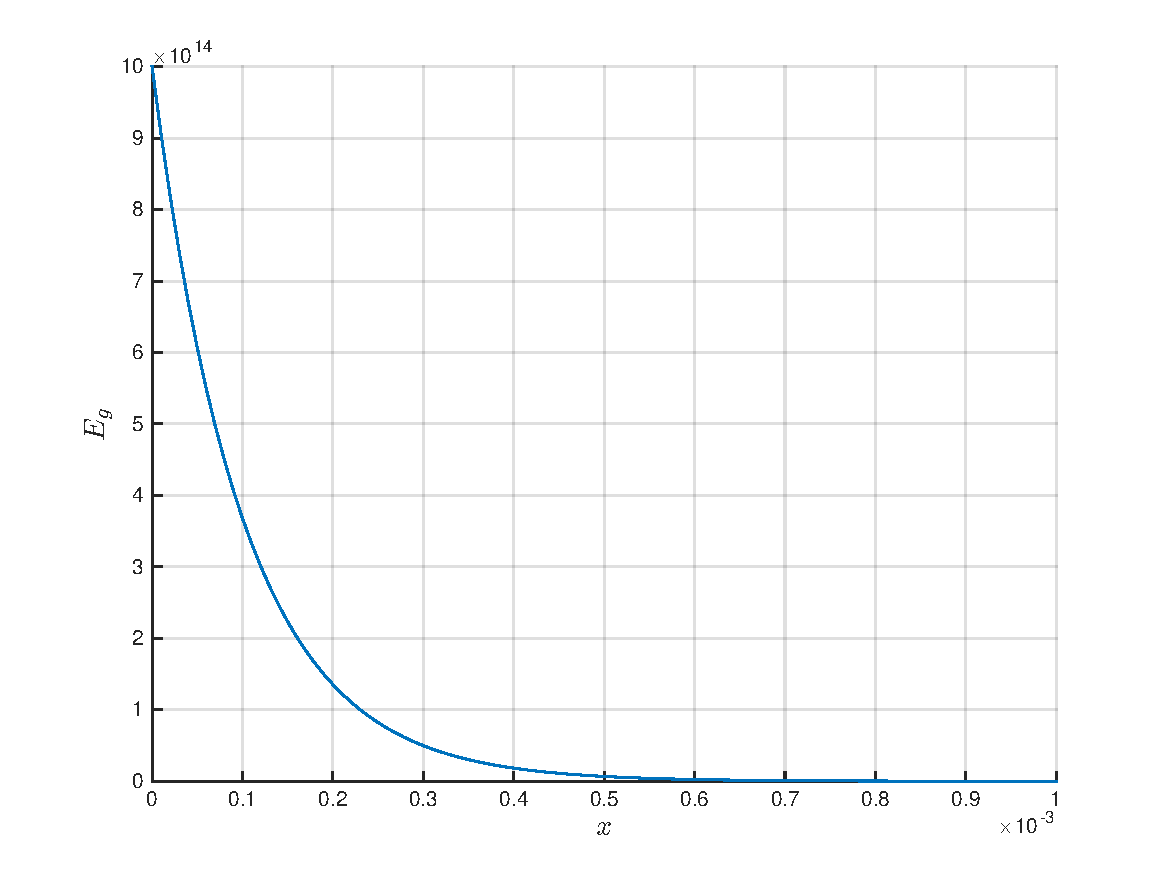
\includegraphics[width = 0.8\textwidth]{plot2.pdf}
			\end{figure}
			The electron flow is directed from the left to the right.\\
			\begin{align*}
				J_{\text{diffusion}_n} &= q D_p \dod{n}{x}\\
				&= \left( 1.6 \times 10^{-19} \si{\coulomb} \right) \left( 25 \si{\centi\metre\squared\per\second} \right) \left( -\frac{10^{15}}{10^{-4}} e^{-\frac{x}{10^{-4}}} \si{\per\centi\metre\tothe{4}} \right)\\
				&= -40 e^{-10^4 x} \si{\ampere\per\centi\metre\squared}
			\end{align*}
			Therefore,
			\begin{align*}
				J_{\text{diffusion}_n}(x = 0) &= -40 e^{0}\\
				&= -40 \si{\ampere\per\centi\metre\squared}\\
				J_{\text{diffusion}_n}(x = L_n = 10^{-4}) &= -40 e^{-1}\\
				&= -14.72 \si{\ampere\per\centi\metre\squared}\\
				J_{\text{diffusion}_n}(x \to \infty) &= -40 \cdot 0\\
				&= 0
			\end{align*}
			\begin{align*}
				n(x) &= 10^{15} e^{-\frac{x}{L_n}} \si{\per\centi\metre\cubed}\\
				\therefore n(0) &= 10^{15} e^{0}\\
				&= 10^{15} \si{\per\centi\metre\cubed}\\
				\therefore n(L_n) &= 10^{15} e^{-1}\\
				&= \frac{10^{15}}{e} \si{\per\centi\metre\cubed}
			\end{align*}
			Therefore, at $x = L_n$, $n(x)$ is $\frac{1}{e}$ of its original value.
	\end{enumerate}
\end{solution}

\begin{question}
	Suppose we use optical absorption and emission as a technique for determining the Al composition of a sample of Al$_x$Ga$_{1 - x}$As.
	A feature of AlGaAs is that it is a material which demonstrates radiative recombination, i.e. it emits photons as a result of carrier recombination.\\
	In our experiment, we illuminate a sample of AlGaAs with a 509 \si{\nano\metre} laser, and the wavelength of photons emitted from the material is 689 \si{\nano\metre}.\\
	Answer the following.
	\begin{enumerate}
		\item
			Is this laser a suitable choice for the experiment?
		\item
			Given the plot below, of $E_{\text{gap}}$ as a function of aluminium composition $x$ in Al$_x$Ga$_{1 - x}$As, what is the value of $x$ in this particular material?
			\begin{figure}[H]
				\centering
				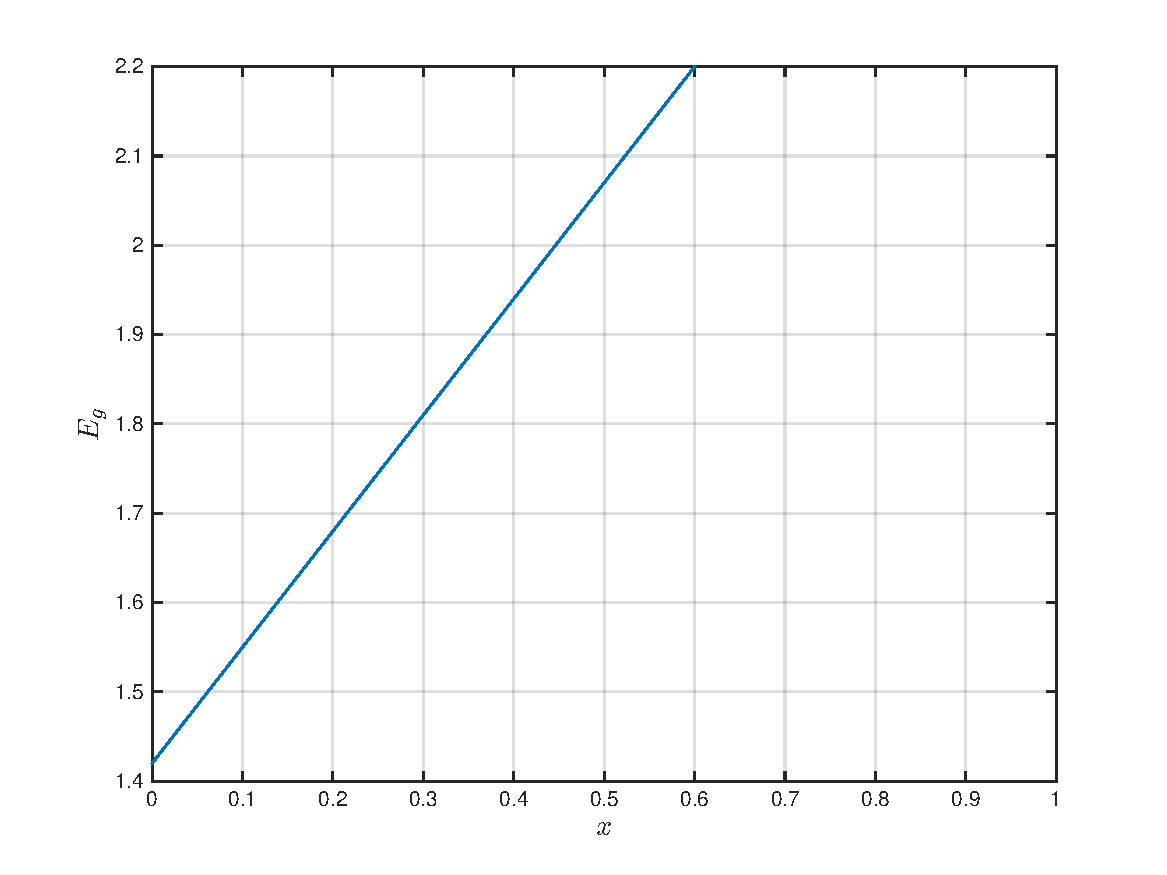
\includegraphics[width = \textwidth]{plot1.pdf}
			\end{figure}
	\end{enumerate}
\end{question}

\begin{solution}
	\begin{enumerate}[leftmargin=*]
		\item
			The wavelength of the laser is less than the wavelength of the photons emitted.
			Therefore, the energy of the photons emitted by the laser is greater than the energy band gap of the sample.
			Hence, the laser is a suitable choice, but a laser which emits photons of lesser energy can also be used, as long as the wavelength of the laser is less than 689 \si{\nano\metre}.
		\item
			\begin{align*}
				E &= \frac{h c}{\lambda}\\
				&= \frac{1.24}{689} \times 10^3\\
				&= 1.8 \electronvolt
			\end{align*}
			Therefore, the value of $x$ in this particular material is approximately 0.3.
	\end{enumerate}
\end{solution}

\begin{question}
	Consider a particle of mass $m$ and the following potential $V(x)$.
	\begin{align*}
		V(x) &= -\alpha \left( \delta(x + a) + \delta(x - a) \right)
	\end{align*}
	We solved in class for the even wave functions.
	Repeat what we did for the odd solutions, i.e. write down the odd wave function, and find the allowed values for $k$.
	Is there an allowed energy for all values of $\alpha$?
\end{question}

\begin{solution}
	\begin{align*}
		V(x) &= -\alpha \left( \delta(x + a) + \delta(x - a) \right)
	\end{align*}
	Therefore,
	\begin{align*}
		\psi(x) &=
			\begin{cases}
				A e^{k x} &;\quad x < -a\\
				B e^{k x} + C e^{-k x} &\quad -a < x < a\\
				D e^{-k x} &;\quad a < x\\
			\end{cases}
	\end{align*}
	where
	\begin{align*}
		k &= \sqrt{-\frac{2 m E}{\hbar^2}}
	\end{align*}
	Therefore,
	\begin{align*}
		\psi(-a + \varepsilon) &= \psi(-a - \varepsilon)\\
		\psi(a + \varepsilon) &= \psi(a - \varepsilon)\\
		\psi'(-a + \varepsilon) - \psi'(-a - \varepsilon) &= -\frac{2 m \alpha}{\hbar^2} \psi(-a)\\
		\psi'(a + \varepsilon) - \psi'(a - \varepsilon) &= -\frac{2 m \alpha}{\hbar^2} \psi(a)
	\end{align*}
	As $V(x)$ is even, the wave function $\psi(x)$ can be split into odd and even parts, i.e. $\psi_{\text{even}}(x)$ and $\psi_{\text{odd}}(x)$.\\
	Therefore, for $\psi_{\text{odd}}(x)$,
	\begin{align*}
		A &= -D\\
		B &= -C
	\end{align*}
	Therefore,
	\begin{align*}
		\psi_{\text{odd}}(x) &=
			\begin{cases}
				A e^{k x} &;\quad x < -a\\
				B \left( e^{k x} - e^{-k x} \right) &;\quad -a < x < a\\
				-A e^{-k x} &;\quad a < x\\
			\end{cases}
	\end{align*}
	Therefore,
	\begin{align*}
		{\psi_{\text{odd}}}'(x) &=
			\begin{cases}
				k A e^{k x} &;\quad x < -a\\
				k B \left( e^{k x} + e^{-k x} \right) &;\quad -a < x < a\\
				k A e^{-k x} &;\quad a < x\\
			\end{cases}
	\end{align*}
	Therefore,
	\begin{align*}
		\psi(-a + \varepsilon) &= \psi(-a - \varepsilon)\\
		\therefore A e^{-k a} &= B \left( e^{- k a} - e^{k a} \right)\\
		\psi'(-a + \varepsilon) - \psi'(-a - \varepsilon) &= -\frac{2 m \alpha}{\hbar^2} \psi(-a)\\
		\therefore k B \left( e^{-k a} + e^{k a} \right) - k A e^{k a} &= -\frac{2 m \alpha}{\hbar^2} A e^{-k a}
	\end{align*}
	Therefore,
	\begin{align*}
		A &= B \left( 1 - e^{2 k a} \right)\\
		B \left( 1 + e^{2 k a} \right) &= A \left( 1 - \frac{2 m \alpha}{\hbar^2 k} \right)
	\end{align*}
	Therefore,
	\begin{align*}
		1 + e^{2 k a} &= \left( 1 - e^{2 k a} \right) \left( 1 - \frac{2 m \alpha}{\hbar^2 k} \right)\\
		\therefore 1 + e^{2 k a} &= 1 - \frac{2 m \alpha}{\hbar^2 k} - e^{2 k a} + e^{2 k a} \frac{2 m \alpha}{\hbar^2 k}\\
		\therefore \frac{m \alpha}{\hbar^2 k} &= e^{2 k a} \left( \frac{m \alpha}{\hbar^2 k} - 1 \right)\\
		\therefore 1 &= e^{2 k a} \left( 1 - \frac{\hbar^2 k}{m \alpha} \right)\\
		\therefore e^{-2 k a} &= 1 - \frac{\hbar^2 k}{m \alpha}\\
	\end{align*}
	Let
	\begin{align*}
		z &= 2 k a\\
		c &= \frac{\hbar^2}{2 a m \alpha}
	\end{align*}
	Therefore,
	\begin{align*}
		e^{-z} &= 1 - c z
	\end{align*}
	Therefore, there exists at least one solution.
\end{solution}

\begin{question}
	Consider a particle of mass $m$, and the following potential.
	\begin{align*}
		V(x) &=
			\begin{cases}
				\infty &;\quad x < -a\\
				\alpha \delta(x) &;\quad -a < x < a\\
				\infty &;\quad a < x\\
			\end{cases}
	\end{align*}
	\begin{enumerate}
		\item
			Sketch the potential.
		\item
			Write down the general from of the wave function for all values of position $x$.
			Indicate the number of unknown parameters and list them.
			Hint: Use $\sin x$ and $\cos x$ functions as for the infinite potential well.
		\item
			Write down the boundary conditions.
		\item
			Find the allowed energies for the particle corresponding to the even wave functions.
			Hint: Even solutions satisfy $\psi(x) = \psi(-x)$.
		\item
			Find the allowed energies for the particle corresponding to the odd wave functions.
			Hint: Even solutions satisfy $\psi(x) = -\psi(-x)$.
		\item
			Compare your answer to the allowed energy states of an infinite well, without a delta function in the middle.
	\end{enumerate}
\end{question}

\begin{solution}
	\begin{enumerate}
		\item
			\begin{align*}
				V(x) &=
					\begin{cases}
						\infty &;\quad x < -a\\
						\alpha \delta(x) &;\quad -a < x < a\\
						\infty &;\quad a < x\\
					\end{cases}
			\end{align*}
			\begin{figure}[H]
				\centering
				\begin{tikzpicture}
					\def\xMIN{-4};
					\def\xMAX{4};
					\def\yMIN{0};
					\def\yMAX{3};

					\def\a{2};
					\def\Alpha{2};

					\newcommand{\drawImpulse}[3]
					{
						\draw [smooth, samples = 1000, domain = \xMIN:\xMAX] plot (\x,{#1*exp(-pow((\x - #2),2)/2*pow(#3,2))})
					}

					\begin{scope}[-stealth]
						\draw (\xMIN,0) -- (\xMAX,0) node [right] {$x$};
						\draw (0,\yMIN) -- (0,\yMAX) node [above] {$V(x)$};
					\end{scope}

					\begin{scope}
						\draw (\xMIN,\yMAX - 1) -- (-\a,\yMAX - 1);
						\drawImpulse{(\yMAX - 1)}{0}{20};
						\draw (\a,\yMAX - 1) -- (\xMAX,\yMAX - 1);
					\end{scope}

					\begin{scope}[dashed]
						\draw (\a,0) node [below] {$a$} -- (\a,\yMAX);
						\draw (-\a,0) node [below] {$-a$} -- (-\a,\yMAX);
					\end{scope}

				\end{tikzpicture}
			\end{figure}
		\item
			Therefore, solving the time independent Schrödinger equation,
			\begin{align*}
				\psi(x) &=
					\begin{cases}
						0 &;\quad x < -a\\
						A e^{i k x} &;\quad -a < x < 0\\
						A e^{-i k x} &;\quad 0 < x < a\\
						0 &;\quad a < x\\
					\end{cases}
			\end{align*}
			where
			\begin{align*}
				k &= \sqrt{\frac{2 m E}{\hbar^2}}
			\end{align*}
			Therefore,
			\begin{align*}
				\psi(x) &=
					\begin{cases}
						0 &;\quad x < -a\\
						A \cos(k x) + B \sin(k x) &;\quad -a < x < 0\\
						A \cos(-k x) + B \sin(-k x) &;\quad 0 < x < a\\
						0 &;\quad a < x\\
					\end{cases}\\
				&=
					\begin{cases}
						0 &;\quad x < -a\\
						A \cos(k x) + B \sin(k x) &;\quad -a < x < 0\\
						A \cos(k x) - B \sin(k x) &;\quad 0 < x < a\\
						0 &;\quad a < x\\
					\end{cases}
			\end{align*}
			Therefore, the unknowns are $A$ and $B$.
		\item
			As $\psi(x)$ is always continuous,
			\begin{align*}
				0 &= A \cos(-k a) + B \sin(-k a)\\
				0 &= A \cos(k a) - B \sin(k a)
			\end{align*}
		\item
			For $\psi_{\text{even}}(x)$,
			\begin{align*}
				B &= 0
			\end{align*}
			Therefore,
			\begin{align*}
				\psi_{\text{even}}(x) &=
					\begin{cases}
						0 &;\quad x < -a\\
						A \cos(k x) + B \sin(k x) &;\quad -a < x < 0\\
						A \cos(k x) - B \sin(k x) &;\quad 0 < x < a\\
						0 &;\quad a < x\\
					\end{cases}
			\end{align*}
			Substituting the boundary condition, for $x = -a$,
			\begin{align*}
				0 &= A \cos(k a) - B \sin(k a)
			\end{align*}
			Substituting the boundary condition, for $x = a$,
			\begin{align*}
				0 &= A \cos(k a) - B \sin(k a)
			\end{align*}
			Therefore,
			\begin{align*}
				A \cos(k a) &= B \sin(k a)\\
				\therefore \tan k a &= \frac{A}{B}
			\end{align*}
			Therefore, solving the boundary conditions for $\psi'$,
			\begin{align*}
				-2 k B &= \frac{2 m \alpha}{\hbar^2} A
			\end{align*}
			Therefore, solving the conditions simultaneously, as for infinite quantum well,
			\begin{align*}
				-\frac{\hbar^2}{m \alpha a} z &= \tan z
			\end{align*}
		\item
			For $\psi_{\text{odd}}(x)$,
			\begin{align*}
				A &= 0
			\end{align*}
			Therefore,
			\begin{align*}
				\psi_{\text{even}}(x) &=
					\begin{cases}
						0 &;\quad x < -a\\
						A \cos(k x) + B \sin(k x) &;\quad -a < x < 0\\
						-A \cos(k x) + B \sin(k x) &;\quad 0 < x < a\\
						0 &;\quad a < x\\
					\end{cases}
			\end{align*}
			For $\psi$ to be continuous at $x = 0$,
			\begin{align*}
				B &= -B\\
				&= 0
			\end{align*}
			Therefore,
			\begin{align*}
				\psi_{\text{even}}(x) &=
					\begin{cases}
						0 &;\quad x < -a\\
						B \sin(k x) &;\quad -a < x < 0\\
						B \sin(k x) &;\quad 0 < x < a\\
						0 &;\quad a < x\\
					\end{cases}
			\end{align*}
			Substituting the boundary condition, for $x = -a$,
			\begin{align*}
				B \sin(k a) &= 0
			\end{align*}
			Substituting the boundary condition, for $x = a$,
			\begin{align*}
				B \sin(k a) &= 0
			\end{align*}
			Therefore,
			\begin{align*}
				k a &= n \pi
			\end{align*}
			Therefore,
			\begin{align*}
				k a &= n \pi
			\end{align*}
			Therefore,
			\begin{align*}
				k_n &= \frac{n \pi}{a}\\
				\therefore \sqrt{\frac{2 m E}{\hbar^2}} &= \frac{n \pi}{a}\\
				\therefore \frac{2 m E}{\hbar^2} &= \frac{n^2 \pi^2}{a^2}\\
				\therefore E &= \frac{\pi^2 n^2 \hbar^2}{2 m a^2}
			\end{align*}
		\item
			For the odd functions, the result is the same as the result for an infinite square well, without a delta function.
			For the even function, the energy levels are slightly different than that for an infinite well without a delta function.
	\end{enumerate}
\end{solution}

\end{document}
